\documentclass[a4paper,14pt]{extreport}
\usepackage[left=1.5cm,right=1.5cm,
    top=1.5cm,bottom=2cm,bindingoffset=0cm]{geometry}
\usepackage{scrextend}
\usepackage[T1,T2A]{fontenc}
\usepackage[utf8]{inputenc}
\usepackage[english,russian,ukrainian]{babel}
\usepackage{tabularx}
\usepackage{amssymb}
\linespread{1.5}
\usepackage{color}
\usepackage{amsmath}
\usepackage{mathrsfs}
\usepackage{listings}
\usepackage{graphicx}
\graphicspath{{./images/} }
\usepackage{lipsum}
\usepackage{xcolor}
\usepackage{hyperref}
\usepackage{tcolorbox}
\usepackage{tikz}
\usepackage[framemethod=TikZ]{mdframed}
\usepackage{wrapfig,boxedminipage,lipsum}
\mdfdefinestyle{MyFrame}{%
linecolor=blue,outerlinewidth=2pt,roundcorner=20pt,innertopmargin=\baselineskip,innerbottommargin=\baselineskip,innerrightmargin=20pt,innerleftmargin=20pt,backgroundcolor=gray!50!white}
 \usepackage{csvsimple}
 \usepackage{supertabular}
\usepackage{pdflscape}
\usepackage{fancyvrb}
%\usepackage{comment}
\usepackage{array,tabularx}
\usepackage{colortbl}

\usepackage{varwidth}
\tcbuselibrary{skins}
\usepackage{fancybox}


\usepackage{tikz}
\usepackage[framemethod=TikZ]{mdframed}
\usepackage{xcolor}
\usetikzlibrary{calc}
\makeatletter
\newlength{\mylength}
\xdef\CircleFactor{1.1}
\setlength\mylength{\dimexpr\f@size pt}
\newsavebox{\mybox}
\newcommand*\circled[2][draw=blue]{\savebox\mybox{\vbox{\vphantom{WL1/}#1}}\setlength\mylength{\dimexpr\CircleFactor\dimexpr\ht\mybox+\dp\mybox\relax\relax}\tikzset{mystyle/.style={circle,#1,minimum height={\mylength}}}
\tikz[baseline=(char.base)]
\node[mystyle] (char){#2};}
\makeatother

\definecolor{ggreen}{rgb}{0.4,1,0}
\definecolor{rred}{rgb}{1,0.1,0.1}
\definecolor{amber}{rgb}{1.0, 0.75, 0.0}
\definecolor{babyblue}{rgb}{0.54, 0.81, 0.94}
\definecolor{asparagus}{rgb}{0.53, 0.66, 0.42}
\definecolor{chartreuse}{rgb}{0.5, 1.0, 0.0}
\definecolor{darkorchid}{rgb}{0.6, 0.2, 0.8}

\usepackage{float}
\usepackage{wrapfig}
\usepackage{framed}
%for nice Code{
\lstdefinestyle{customc}{
  belowcaptionskip=1\baselineskip,
  breaklines=true,
  frame=L,
  xleftmargin=\parindent,
  language=C,
  showstringspaces=false,
  basicstyle=\small\ttfamily,
  keywordstyle=\bfseries\color{green!40!black},
  commentstyle=\itshape\color{purple!40!black},
  identifierstyle=\color{blue},
  stringstyle=\color{orange},
}
\lstset{escapechar=@,style=customc}
%}


\begin{document}
\pagecolor{white}

%----------------------------------------1
\newtcbox{\xmybox}[1][red]{on line, arc=7pt,colback=#1!10!white,colframe=#1!50!black, before upper={\rule[3pt]{0pt}{10pt}},boxrule=1pt,boxsep=0pt,left=6pt,right=6pt,top=2pt,bottom=2pt}


\begin{center}Bohdan Lyshchenko DP-82 Variant №4
\vspace{1cm}

\end{center}


\begin{center}Поясніть закон сталості теплоємності. У чому полягає модель Ейнштейна для опису теплоємності?\end{center}

The law of constancy of heat capacity is an empirical law according to which the molar heat capacity of different solids at room temperature is the same:
$$ C_{\text{тв.т}} = 3R $$
where R is a universal gas constant. Important is the fact that the molar heat capacity of a solid at normal and elevated temperatures is twice the heat capacity of the gas: Сгаз = 3/2 R, а (it should be remembered that in one mole of the test substance the gas has the same number of atoms as the solid body is Avogadro's number $ N_A $ = 6.02 $ \cdot 10 ^{23} $ mol $ ^{- 1} $). \\

According to classical statistics (ie statistical physics based on classical mechanics), for each degree of freedom of the particle in the molar heat capacity of the gas is the value of R / 2; this rule is called the law of equal distribution. The monoatomic gas particle has only three degrees of freedom, so the molar heat capacity of the gas should be 3/2 R (ie about 12.5 j / Kmol $ \cdot $ K), or 3 cal / (mol $ \cdot $ deg)], which agrees well with the experiment. \\

The reason is that free gas atoms have only kinetic energy: each gas atom has 3 degrees of freedom, and for each degree
freedom accounts for $ kBT / $ 2 of energy, ie only 3/2 $ k_{B} $ T per
atom; since in one mole of NA atoms, the molar heat capacity of the gas
is equal to 3/2 R (k - Boltzmann constant - determines the relationship between temperature and
energy, k = 1.4 $ \cdot 10 ^{23} $ J / K = 8.6 $ \cdot 10 ^{- 5} $ eV / K) \\

The atom connected in the lattice of the crystal during its oscillations has not only kinetic but also equal (on average) potential energy, ie the atom in the lattice has twice as much energy: 3 kT. It follows from this that the law of constancy of heat capacity: $ C_{\text{tvt}} $ = 3R. This Dulong-Petit law in the dynamic formulation of the problem is derived in the assumption that the crystal lattice of a body consists of atoms, each of which makes harmonic oscillations in three directions due to the lattice structure, and oscillations in different directions are independent of each other. It turns out that each atom represents three oscillators with energy E due to the following formula: \\
$$ E = kT $$

\begin{figure}[h]
\center{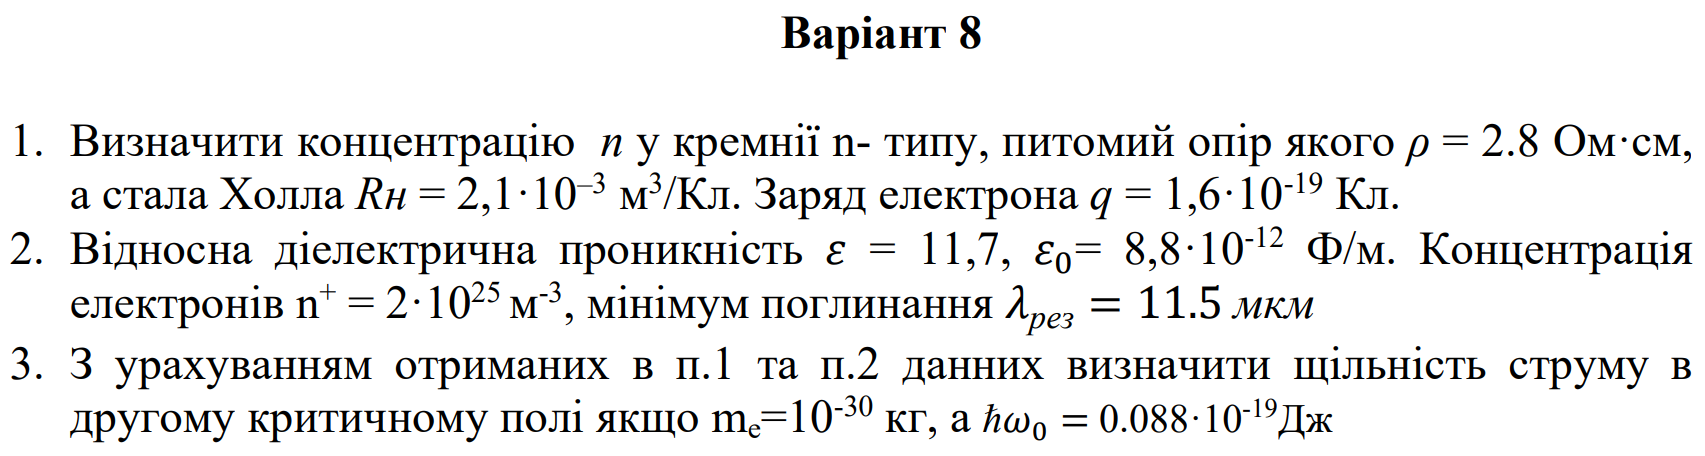
\includegraphics[width=0.6\linewidth]{1.png}}
\caption{dependence of molar heat capacity on temperature: 1 - for ideal gas, 2 - lattice heat capacity of solids}
\label{ris1}
\end{figure}

This formula follows from the theorem on the equal distribution of energy by degrees of freedom. Each oscillator has one degree of freedom, and therefore its average kinetic energy is kT / 3. Since the oscillations occur harmonically, the average potential energy is equal to the average kinetic energy, and the total energy is equal to their sum. The number of oscillators in one mole of matter is 3NA, and their total energy is numerically equal to the heat capacity of the body - hence the law of constancy of thermal conductivity. \\

Quantum theory of Einstein's heat capacity. The main assumption of the theory is that the atomic oscillator in the crystal lattice is quantum, not classical. In addition, as in the previous model, the oscillators are considered independent.
The energy of a quantum oscillator with frequency $ \omega $ is absorbed (or radiated) only in portions - quanta $ hv = \hbar \omega $. Schematically, this is shown in Fig. 2 (diagram on the left).


\begin{figure}[h]
\center{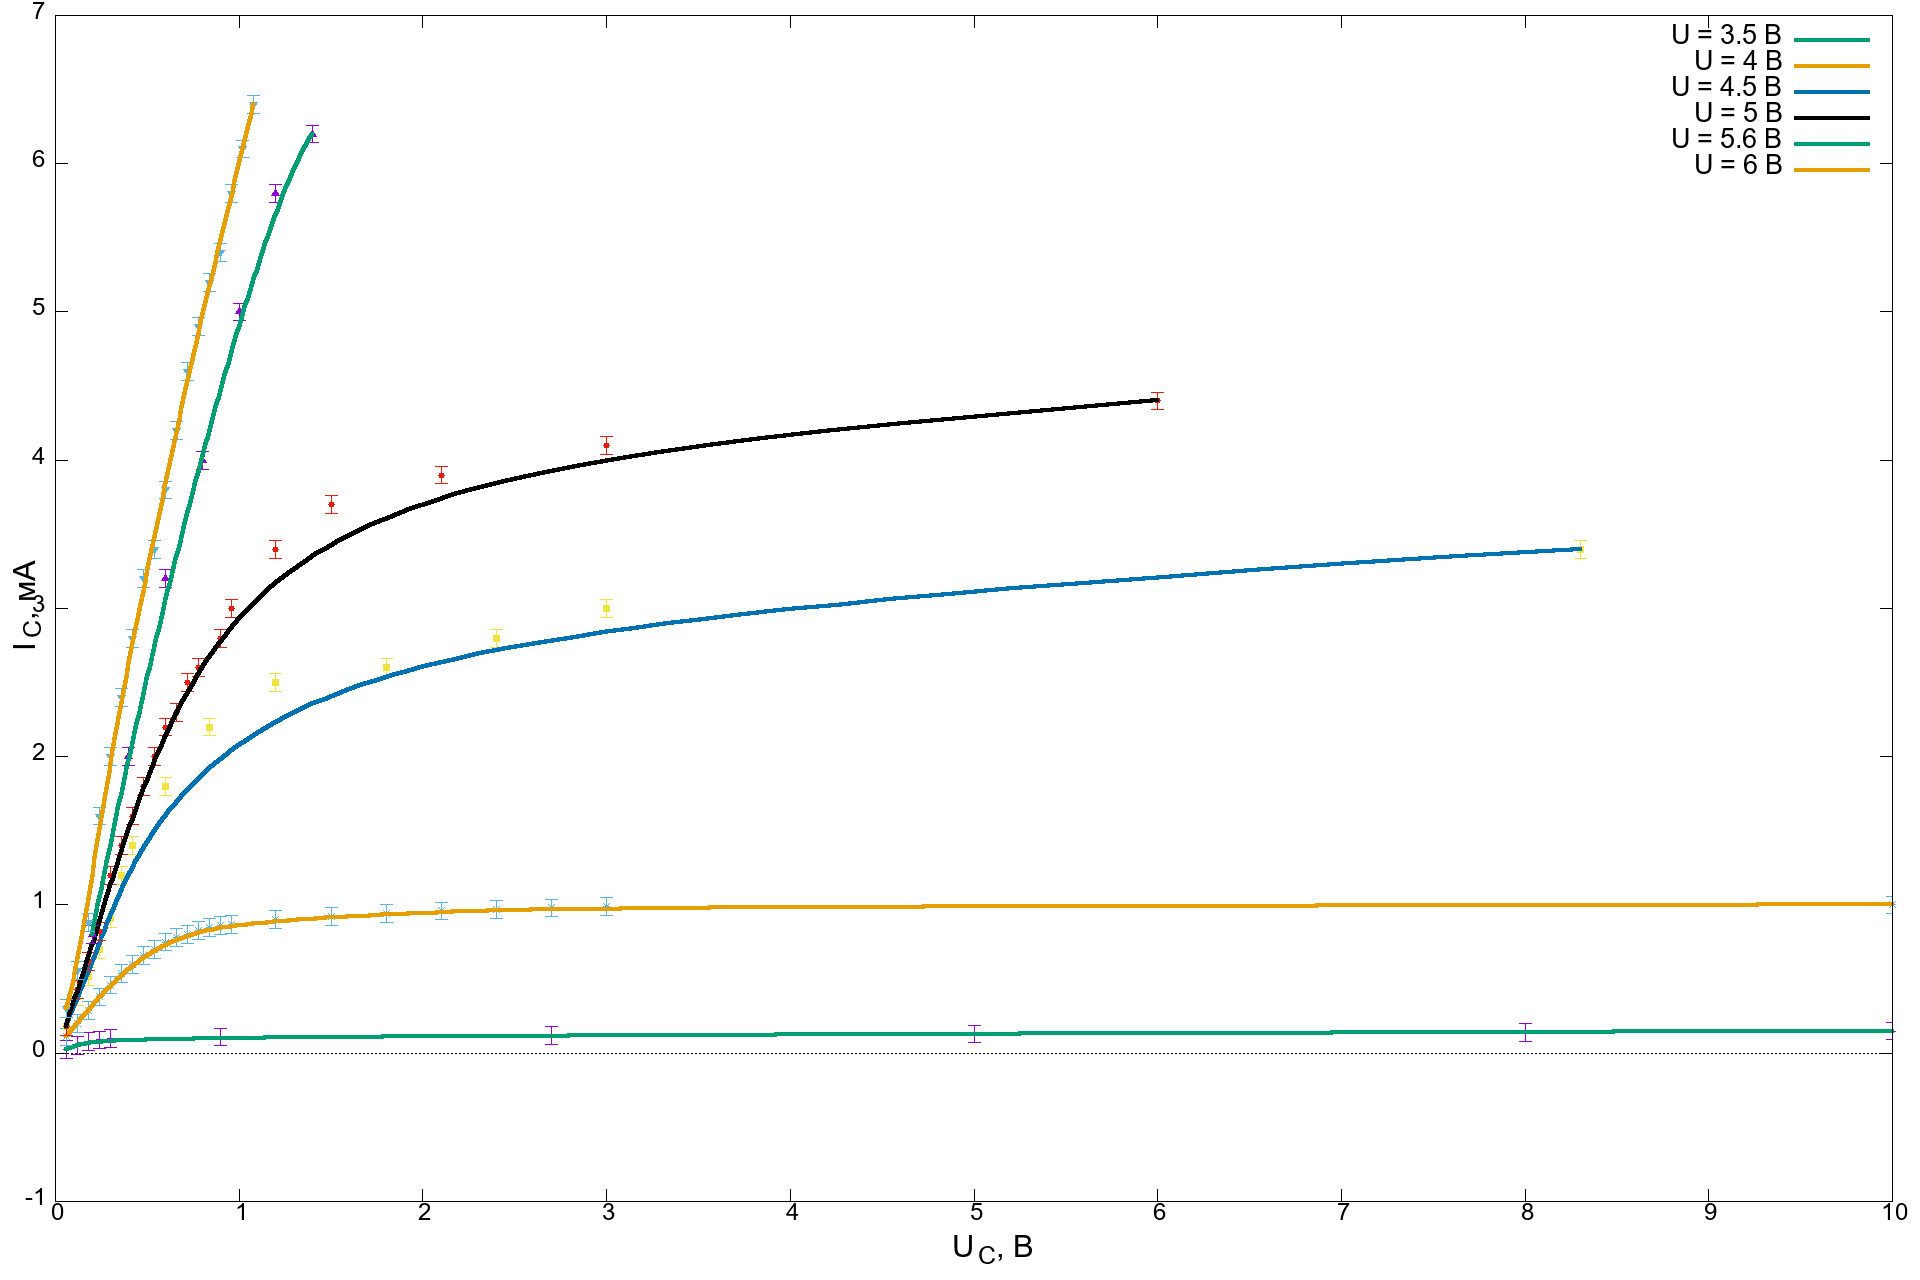
\includegraphics[width=0.6\linewidth]{2.png}}
\caption{Comparison of the quantum model of heat capacity of independent oscillators (curve 1) and the model of coupled oscillators (curve 2)}
\label{ris1}
\end{figure}


In the case of a relatively high temperature T3, when the thermal motion is more intense and the average thermal energy of the lattice (kT3) is much higher than the energy quantum of the oscillator (kT3 >> $ \hbar \omega $), and the fact that the oscillator is quantum is not significant, and therefore, the classical Dulong-Petit law holds.
However, in the case of low temperature, the average energy of thermal motion is approximately the same as the energy of the quantum oscillator: kT1 $ \approx \hbar \omega $. Of course, the distribution of energy between the oscillations of the lattice is chaotic, but an increasing number of quantum oscillators do not perceive (and do not emit) energy, ie heat capacity should decrease with decreasing temperature.
  This is the result obtained by Einstein. His theory was based on the assumption that the atoms in the crystal lattice behave like harmonic oscillators that do not interact with each other (and therefore the oscillation frequency of all oscillators is the same). The number of oscillators in 1 mole of matter is $ 3N_A $ and their energy is quantized. According to the model proposed by Einstein, near the temperature of absolute zero, the heat capacity goes to zero, and at high temperatures, on the contrary, the Dulong-Petit law holds.
  











\end{document}